\documentclass{beamer}
\usetheme{Berlin}

\usepackage[polish]{babel}
\usepackage[utf8]{inputenc}
\usepackage[T1]{fontenc}
\usepackage{multirow}
\usepackage{graphicx}
\graphicspath{ {./images/} }

\title{Drzewa}
\author{Dominik Belgrau}
\begin{document}

\begin{frame}
\titlepage
\end{frame}

\begin{frame}{Podział}
\begin{table}
\begin{center}
\begin{tabular}{ |p{3cm}|p{3cm}| }
 \hline
 \multicolumn{2}{|c|}{Typ} \\
 \hline
 Liściaste &Iglaste\\
\hline
\end{tabular}
\caption{Drzewa}
\label{t1}
\end{center}
\end{table}
\end{frame}

\begin{frame}{Liściaste}
\begin{enumerate}[a)]
\item Dąb
\pause
\item Klon
\pause
\item Kasztanowiec
\end{enumerate}
\end{frame}

\begin{frame}{Dab}
\begin{figure}[h!]
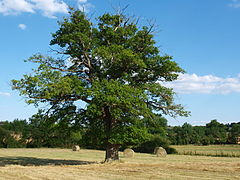
\includegraphics[scale=13]{dab.jpg}
\caption{Dąb \cite{Wiki}}
\label{dab}
\end{figure}
\end{frame}

\begin{frame}{Klon}
\begin{figure}[h!]
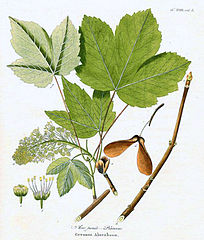
\includegraphics[scale=2]{klon.jpg}
\caption{Klon \cite{Wiki}}
\label{klo}
\end{figure}
\end{frame}

\begin{frame}{Kasztanowiec}
\begin{figure}[h!]
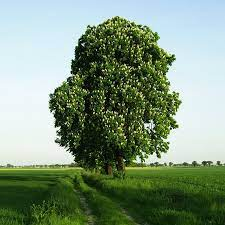
\includegraphics[scale=0.7]{kasz.jpg}
\caption{Kasztanowiec \cite{Wiki}}
\label{kas}
\end{figure}
\end{frame}

\begin{frame}{Iglastee}
\begin{enumerate}[a)]
\item Jodła
\pause
\item Sosna
\pause
\item Limba
\end{enumerate}
\end{frame}

\begin{frame}{Jodła}
\begin{figure}[h!]
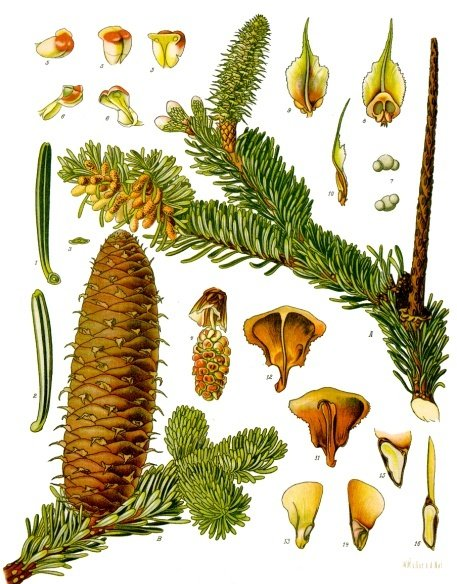
\includegraphics[scale=0.3]{jod.jpg}
\end{figure}
\end{frame}

\begin{frame}{Sosna}
\begin{figure}[h!]
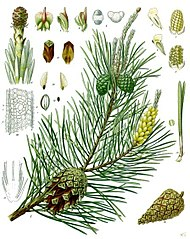
\includegraphics[scale=0.7]{sos.jpg}
\end{figure}
\end{frame}

\begin{frame}{Limba}
\begin{figure}[h!]
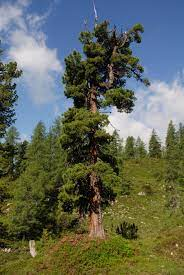
\includegraphics[scale=0.6]{lim.jpg}
\end{figure}
\end{frame}

\begin{frame}{Odwołania}
Wszystko dzięki \cite{Miotk}
\begin{enumerate}[a)]
\item Tabela \ref{t1} pokazuje podział drzew.
\pause
\item Obraz \ref{dab} pokazuje dąb.
\pause
\item Obraz  \ref{klo} pokazuje klon.
\pause
\item Obraz \ref{kas} pokazuje kasztanowca.
\end{enumerate}
\end{frame}

\begin{frame}{Bibliografia}
\section{Bibliografia}\label{bb}
\begin{thebibliography}{2}
\bibitem{Miotk}
M. Miotk "Wprowadzenie do klasy Beamer w \LaTeX \footnote[1]{Taki język śmieszny}"
\bibitem{Wiki}
Zdjęcia: wikipedia.org\footnote[2]{Taka strona w internetach}
\end{thebibliography}
\end{frame}

\end{document}
